\documentclass[AMS,STIX1COL]{WileyNJD-v2}

\def\tightlist{}

%\usepackage{amsmath,amsfonts}

\articletype{Article Type}%

\received{26 April 2016}
\revised{6 June 2016}
\accepted{6 June 2016}

\raggedbottom

\begin{document}

\title{This is the sample article title\protect\thanks{This is an example for title footnote.}}

\author[1]{Author One*}

\author[2,3]{Author Two}

\author[3]{Author Three}

\authormark{AUTHOR ONE \textsc{et al}}


\address[1]{\orgdiv{Org Division}, \orgname{Org Name}, \orgaddress{\state{State name}, \country{Country name}}}

\address[2]{\orgdiv{Org Division}, \orgname{Org Name}, \orgaddress{\state{State name}, \country{Country name}}}

\address[3]{\orgdiv{Org Division}, \orgname{Org Name}, \orgaddress{\state{State name}, \country{Country name}}}

\corres{*Corresponding author name, This is sample corresponding address. \email{authorone@gmail.com}}

\presentaddress{This is sample for present address text this is sample for present address text}

\abstract[Summary]{
In many machine learning applications, the observed data is a
discretely-sampled realisation of a continuous process. While one can
naively treat such data as vectors in Euclidean space, one may do better
to regard them as functional data.  
When the underlying curves of interest lie on a manifold, e.g.~probability density
functions or warped curves of a common template function, there is further structure to exploit. 
This work addresses the estimation of pairwise geodesic
distances between functional manifold data that are observed with noise,
causing them to lie off the manifold. This setting falls outside of
classic manifold learning techniques which require data to live exactly
on or very near a manifold. The proposed methodology first sends the
observed functional data to the hidden manifold, estimated using
subspace-constrained mean-shift. Geodesic distances are subsequently
calculated by employing shortest-path algorithms on this estimated
manifold. Improved estimation of the pairwise geodesic distance has
potential benefits for downstream tasks such as distance-based functional classification.
}

\keywords{keyword1, keyword2, keyword3, keyword4}

\jnlcitation{\cname{%
\author{Williams K.}, 
\author{B. Hoskins}, 
\author{R. Lee}, 
\author{G. Masato}, and 
\author{T. Woollings}} (\cyear{2016}), 
\ctitle{A regime analysis of Atlantic winter jet variability applied to evaluate HadGEM3-GC2}, \cjournal{Q.J.R. Meteorol. Soc.}, \cvol{2017;00:1--6}.}

\maketitle

\footnotetext{\textbf{Abbreviations:} ANA, anti-nuclear antibodies; APC, antigen-presenting cells; IRF, interferon regulatory factor}

\newcommand {\To}{\rightarrow}
\newcommand {\TO}{\Rightarrow}
\newcommand {\R}{\mathbb{R}}
\newcommand {\Prob}{\mathbb{P}}
\newcommand{\E}{\mathbb{E}}
\newcommand {\cov}{\textrm{Cov}}
\newcommand {\var}{\textrm{Var}}
\newcommand {\1}{\textrm{\textbf{1}}}
\newcommand{\M}{\mathcal{M}}


\section{INTRODUCTION}\label{introduction}

Many statistical and machine learning methods rely on some measure of
distance. For example, clustering and classification of functional data,
discretely-sampled curves varying over a continuum, is a common learning
task in which distance plays a crucial role. In a naive treatment, the
data may be simply processed as vectors in Euclidean space. Doing so
however risks losing the richness of functional data; indeed, one may do
better to regard the data as functions. The challenge of analyzing
infinite-dimensional objects can be ameliorated if the curves are smooth
since the dimensionality is then only artificially high. This insight
underpins functional data analysis, a subfield of statistics that
studies functional data.

In this work, we advocate that for functional manifold data,
i.e.~functional data that lie on a manifold, the geodesic distance is
more appropriate than the \(L^2\) distance. Indeed, when the manifold
hypothesis is plausible, e.g.~for classes of probability density
functions and classes of warped curves of a common template function,
clustering and classification using the geodesic distance may give
better results than using the \(L^2\) distance.

The manifold setting presents certain challenges since, for nonlinear
manifolds, even basic operations such as addition and subtraction
require special consideration. We will carefully lay out a technique for
estimating the geodesic distance between noisy functional manifold data.

Let \(X_1,\ldots,X_n\) be a sample of \(n\) independent realizations of
a random variable \(X\) that takes value in the Hilbert space
\(L^2([a,b],\R)\). Suppose additionally that the function \(X\) belongs
to a Riemannian manifold \(\M \subset L^2([a,b],\R)\) with Riemannian
metric tensor \(g\) which are often used to assign a metric on the
manifold as follows \cite{Lin2014}. For each point \(X\) on the
manifold, the Riemannian metric tensor \(g\) has an inner product
\(g_X\) on the tangent space \(T_X \M\). The norm of a tangent vector
\(V \in T_X \M\) is defined as \[\|V\| = \sqrt{g_X(V,V)}.\] The geodesic
distance between two functions \(X_i,X_j\) on the manifold \(\M\), based
on this metric tensor \(g\), is defined as
\[ d_{\M}(X_i,X_j):=\inf_{\gamma:[0,1] \to \M, \gamma(0) = X_i, \gamma(1) = X_j} l(\gamma),\]
where
\[ l(\gamma) := \int_0^1 \left\| \frac{\,d\gamma}{\,d t}(t) \right\| \,dt\]
is the length of the piecewise-smooth curve \(\gamma\).

Ideally, the functions \(X_i\) and \(X_j\) are observed on a very dense
domain grid with no measurement error. Then the geodesic distance
\(d_\M(X_i,X_j)\) can be estimated using any of a variety of
shortest-path algorithms, e.g.~the Floyd-Warhsall \cite{Floyd1962}
algorithm. However, most shortest-path algorithms critically assume
observations live near the manifold with little noise \cite{Yeh2005} and
are thus likely to fail for functional data which can be observed with
low signal-to-noise ratio. In this work, we put forth a technique for
the recovery of the \(n{\times}n\) matrix \(G\) of pairwise geodesic
distances: \[
G(i,j)=G(j,i) = \begin{cases} 
      d_{\M} (X_i,X_j) & \textrm{if $i\neq j$,} \\
      0 & \textrm{otherwise.}
   \end{cases}
\] In lieu of \(X_i\) and \(X_j\), we have access only to
discretely-sampled noisy functional observations \(Y_i\) and \(Y_j\)
that possibly lie off the true manifold.

The work of \cite{ChenMuller2012} was among the first in functional data
analysis to consider the manifold hypothesis for functional data. A
notion of the mean and variation of functional manifold data was
introduced there. Of particular relevance to this work is their proposed
P-ISOMAP procedure which allows for noisy functional observations. This
is in contrast to the classic ISOMAP algorithm \cite{Tenenbaum2000}
which assumes observations lie exactly on the manifold. This drawback to
ISOMAP was also realised in \cite{Dimeglio2014} who proposed a procedure
we will call robust-ISOMAP for functional data that is less sensitive to
outliers. We will discuss P-ISOMAP and robust-ISOMAP in more details
below.

\section{RELATED WORK}

\section{PROPOSED METHOD FOR ESTIMATING GEODESIC
DISTANCES}\label{proposed-method-for-estimating-geodesic-distances}

Suppose that each curve \(X_i \in (\M,g)\) is observed with measurement
error on a time grid
\(T_i=(t_{i1},\ldots,t_{iK}), a \le t_{i1} < \ldots < t_{iK} \le b\),
i.e.~we observe a sample of \(K\)-dimensional vectors \(Y_1,\ldots,Y_n\)
with \(Y_{ij} = X_i(t_{ij}) + \epsilon_{ij}\). Let the random variables
\(\epsilon_{ij}\) have mean zero and be uncorrelated with each other. We
assume that each observation grid \(T_1,\ldots,T_n\) is dense,
i.e.~\(K\) is large.

We begin by converting the discretely-sampled functional observations
into continuous ones. Let \(\tilde X_1,\ldots,\tilde X_n\) denote the
functional versions of the raw data obtained by some smoothing method.
For example, we may employ spline smoothing \cite{Ramsay2005} to recover
the functional versions of the raw data, i.e.\\

\begin{equation}\label{eq_spline_smoothing} 
\tilde X_i = \arg \min_{f\in C^2[0,1]}\left\{\sum_{j=1}^{K}\left(f(t_{ij})-Y_{ij}\right)^2+\lambda \|\partial^2_tf\|^2_{L^2}\right\},
\end{equation}

where \(\lambda>0\) is a tuning parameter controlling the smoothness of
\(\tilde X_i\). Our method is based on the idea that the underlying
functional manifold \(\M\) can be sufficiently well-recovered by the
subspace-constrained mean-shift (SCMS) algorithm \cite{Ozertem2011}
which we now review briefly in the Euclidean case. Suppose
\(Z_1,\ldots,Z_n\) is a sample of realisations of a random vector
\(Z \in \M\). We can use a kernel density estimator \(\hat f\) based on
this data to estimate the probability density function of \(Z\). Let the
set \(\hat M\) be comprised of the basins of attraction of \(\hat f\).
The SCMS algorithm sends each point \(Z_i\) to its destination in
\(\hat M\). Theoretical justification that \(\hat M\) as estimated by
SCMS is a reasonable surrogate for the true manifold \(\M\) can be found
in \cite{Genovese2014}.

Before presenting our procedure, we also need to review the ISOMAP
algorithm \cite{Tenenbaum2000}, a three-step procedure that takes as
input a set of points \(x_1,\ldots,x_n\) in a submanifold
\(\M \subset \R^D\) and produces an embedding in the space \(\R^d\) with
\(d<D\) that preserves pairwise geodesic distances. The procedure is as
follows.

\begin{enumerate}
\def\labelenumi{\arabic{enumi}.}
\tightlist
\item
  Construct a weighted graph \(\mathcal{G}\) with nodes corresponding to
  the observations \(x_1,\ldots,x_n\in \R^D\). Two nodes \(x_i\) and
  \(x_j\) are connected by an edge \(e_{ij}\) with weight
  \(d_{ij} 1\{d_{ij} \le \varepsilon \}\) where
  \(d_{ij}=\|x_i-x_j \|_{2}\) and \(\varepsilon > 0\).
\item
  Estimate the pairwise geodesic distances \(d_\M(x_i,x_j)\) based on
  \(\mathcal{G}\) using shortest-path algorithms. Specifically, this is
  the sum of the weights of the edges forming the shortest path, which
  is calculated either with the Floyd-Warshall algorithm
  \cite{Floyd1962} or with the Dijkstra algorithm
  \cite{Dijkstra59anote}.
\item
  Use multidimensional scaling to obtain an embedding in \(\R^d\) that
  preserves the pairwise geodesic distances estimated above.
\end{enumerate}

Note that shortest-path algorithms such as the Floyd-Warshall algorithm
are used to find the smallest path \textit{given} a weighted graph but
they do not produce the weighted graphs themselves. Both P-ISOMAP and
robust-ISOMAP are modifications of ISOMAP in the sense that they change
the construction of the weighted graph in step 1 above.

In what follows, we call IsoGeo the two-step procedure which performs a
modified version of the first step of ISOMAP followed by the original
second step of ISOMAP. The first step of IsoGeo constructs a weighted
graph \(\mathcal{G}\) according to \cite{Dimeglio2014} as follows. First
we construct a complete weighted graph \(\mathcal{G}_c\), meaning that
every pair of nodes \(x_i\) and \(x_j\) is connected by an edge of
weight \(d_{ij}\), so that the graph is independent of the tuning
parameter \(\varepsilon\). Next, we obtain the minimal spanning tree
associated with \(\mathcal{G}_c\) and denote its set of edges by
\(E_s\). The graph \(\mathcal{G}\) is obtained by adding all edges
\(e_{ij}\) to \(E_s\) for which the following condition is true:
\[ \overline{x_ix_j} \subset \bigcup_{i=1}^n B(x_i,\varepsilon_i),\]
where \(B(x_i,\varepsilon_i)\) is the open ball of center \(x_i\) and
radius \(\epsilon_i = \max_{e_{ij}\in E_s}d_{ij}\), and
\(\overline{x_ix_j}= \{x\in R^D \ | \ \exists \lambda \in [0,1], x=\lambda x_i + (1-\lambda)x_j \}\).
Let the distance estimated by IsoGeo be denoted
\(\text{IsoGeo}(x_i,x_j)\). Note that IsoGeo has no tuning parameters.

We are now ready to describe our procedure. Since SCMS is based on
kernel density estimation, we first reduce the dimension of our data
with multidimensional scaling before applying SCMS to avoid the curse of
dimensionality.

\begin{enumerate}
\def\labelenumi{\arabic{enumi}.}
\tightlist
\item
  Discretise the functions \(\tilde X_1,\ldots,\tilde X_n\) by
  evaluating them on a dense common grid
  \(\tilde T=(t_{1},\ldots,t_{D})\). Let \(s\) be a positive integer,
  much smaller than \(D\). Obtain
  \(\tilde X^s_1,\ldots,\tilde X^s_n \in \mathbb R^s\) using
  multidimensional scaling so that the pairwise \(\mathbb R^D\)
  Euclidean distances of the discretised functions \(\tilde X_i\) can be
  preserved as much as possible.
\item
  Apply the subspace constrained mean-shift algorithm \cite{Ozertem2011}
  to each of \(\tilde X^s_i\) to obtain its destination
  \(\tilde X^{s,\hat \M}_i\).
\item
  Our geodesic distance estimator is the \(n{\times}n\) matrix
  \(\hat G\) whose elements are given by \[
  \hat G(i,j)=\hat G(j,i) = \left\{ \begin{array}{ll}
   \text{IsoGeo}(\tilde X^{s,\hat \M}_i,\tilde X^{s,\hat \M}_j) & \textrm{if $i\neq j$,}\\
   0 & \textrm{otherwise.}
    \end{array} \right.
  \]
\end{enumerate}

There are two tuning parameters to our procedure. First, there is the
dimension \(s\) in step 1. In our simulations we try
\(s \in \{1,2,3\}\). The other parameter is the bandwidth \(h\) in the
subspace constrained mean-shift. In our simulations we set \(h\)
according to the heuristic in Equation (A1) of \cite{ChenHo2015}:
\[h = \left(\frac{4}{s+2}\right)^{\frac{1}{s+4}}n^{\frac{-1}{s+4}}\sigma_{\min}, \]
where \(\sigma_{\min}\) is the minimum over \(j=1,\ldots,s\) of the
standard deviation of \(\tilde X^s_{1,j},\ldots, \tilde X^s_{n,j}\),
with \(\tilde X^s_{i,j}\) being the \(j\)th entry of the vector
\(\tilde X^s_{i}\). In reality, depending on the downstream task, both
\(s\) and \(h\) can be tuned in a data-adaptive way, say using
cross-validation.

\section{SIMULATION STUDY}\label{simulation-study}

We perform simulations to study various estimators of pairwise geodesic
distances. We compare the performance of our method to each of the
following four alternatives. The first alternative, denoted \textbf{RD},
takes the naive approach of applying IsoGeo directly on the raw vectors
\(Y_1,\ldots,Y_n \in R^K\). Note that this procedure is only sensible if
all the time grids \(T_1,\ldots,T_n\) are the same.

For the next two alternatives, we first smooth the discretely-sampled
noisy functional data using splines as described in
(\ref{eq_spline_smoothing}). Then, we either estimate pairwise distance
between the smoothed \(\tilde X_1,\ldots,\tilde X_n\) evaluated on a
common time grid of \(D\) points using IsoGeo or the \(L^2\) distance.
The former method will be denoted \textbf{Spline IsoGeo} and the latter
\textbf{Spline L2}.

The final alternative we consider is P-ISOMAP which is the two-step
procedure developed in \cite{ChenMuller2012} for handling noisy
functional data. In the first step, a penalty is incorporated to
robustify the construction of the weighted graph. This is followed by
the original second step of ISOMAP.

The code for P-ISOMAP was provided by \cite{ChenMuller2012} in MATLAB.
We ran P-ISOMAP and tuned for the parameter \(\varepsilon\) and the
penalty parameter \(\delta\) using the relative Frobenius assessment
metric, described below. We found that the penalty parameter chosen in
this oracle fashion was always zero, thus reducing the P-ISOMAP
procedure to standard ISOMAP. Given this, we did not make further
comparison to P-ISOMAP in our simulation study. We also do not present
the results for the RD method which always produced poor estimates of
the geodesic distance.

Three different metrics are used to assess the quality of a pairwise
geodesic distance estimator. The first metric assesses near-\(\epsilon\)
isometry, which we define as the percentage of estimated pairwise
geodesic distances between \(1-\epsilon\) and \(1+\epsilon\) of the
corresponding true pairwise geodesic distance. We form the receiver
operating curve with \(\epsilon\) on the \(x\)-axis and
near-\(\epsilon\) isometry on the \(y\)-axis. The metric is the area
under this receiver operating curve. Thus a good estimator has high
values for the near-isometry metric.

The second metric \(\|G-\hat G\|/\|G\|\) is the Frobenius norm of the
estimation error matrix \(G-\hat G\), relative to the Frobenius norm of
the true distance matrix \(G\). The third metric is the Pearson
correlation coefficient between the upper diagonal of \(G\) and
\(\hat G\). A good geodesic distance estimator has low Frobenius norm
and high Pearson correlation coefficient.

We shall consider three functional manifolds in our simulation study.
Throughout, we make use of a helpful property of one-dimensional
manifolds. If \(X \in \M\), with the \(L^2\) metric tensor, depends on a
scalar parameter \(\theta \in \mathbb R\), then \[
d_\M(X_{\theta_1},X_{\theta_2}) = \int_{\theta_1}^{\theta_2} \left\| \frac{\partial X}{\partial \theta}(t)\right\|_{L^2} \,d\theta.
\]

We also need to make a disclaimer about our sampling technique below.
Proper sampling from a manifold remains an open problem. Even in the
Euclidean case, it is not obvious how sampling should be done
\cite{Diaconis2013}. For now, to safeguard against sampling unevenly on
the functional manifold, we sample on a very narrow support of the
manifold parameters.

\subsection{Isometric functional manifold of normal density
functions}\label{isometric-functional-manifold-of-normal-density-functions}

We take Manifold 2 in \cite{ChenMuller2012} and set the variance of the
normal density to be \(1\). Let \(X_\beta: [a,b] \to \R\) be given by
\(X_\beta(t) = \frac{1}{\sqrt{2\pi}} \exp{[-\frac{1}{2}(t-\beta)^2]}\).
Consider
\[\M = \left \{X_\beta: \beta \in [-1,1], t \in [a,b]\right \},\] with
the \(L^2\) inner product as the metric tensor. First, note that the
``straight'' line connecting \(X_{\beta_1}\) and \(X_{\beta_2}\) does
not always stay inside of \(\M\). Thus the geodesic distance will not
coincide with the \(L^2\) distance.

\begin{figure}
\centering
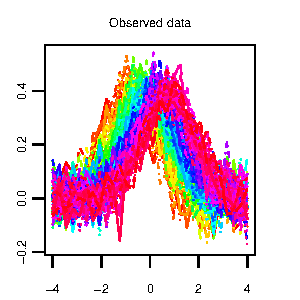
\includegraphics[width=0.3\textwidth]{./graphics/sim_sce=2}
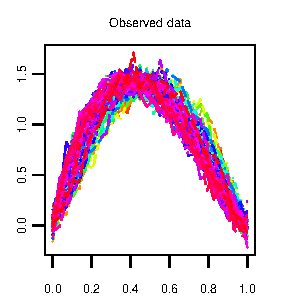
\includegraphics[width=0.3\textwidth]{./graphics/sim_sce=4}
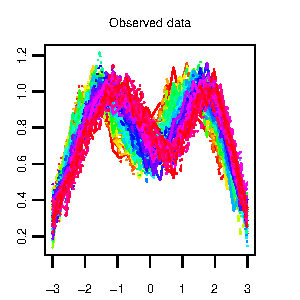
\includegraphics[width=0.3\textwidth]{./graphics/sim_sce=5}
\caption{One hundred noisy curves in the functional manifold of normal probability density.}
\label{fig:sce2} %previous labels {fig:sce4} and {fig:sce5} need to be updated
\end{figure}

We set \(a=-4\) and \(b=4\) and sample \(\beta\) according to a
truncated standard normal with support on \([-1,1]\). The geodesic
distance between the curves \(X_{\beta_1}\) and \(X_{\beta_2}\) is given
by

\begin{eqnarray*}
d_\M(X_{\beta_1},X_{\beta_2}) &=& \int_{\beta_1}^{\beta_2} \left \| \frac{d X_\beta (t)}{d\beta} \right\|_{L^2} d\beta \\
% &=&  \int_{\beta_1}^{\beta_2} \sqrt{ \frac{1}{2\sqrt{\pi}} \int_{-4}^4 \frac{1}{\sqrt{\pi}} \exp\{-(t-\beta)^2\}(t-\beta)^2 dt  }  \  d\beta \\ 
&=&   \int_{\beta_1}^{\beta_2} \sqrt{ \frac{1}{2\sqrt{\pi}} \int_{-4}^4(t-\beta)^2 f(t) dt  }  \  d\beta   \\
&\approx&  \int_{\beta_1}^{\beta_2}  \sqrt{ \frac{1}{2\sqrt{\pi}} \frac{1}{2}} \ d\beta \\
&=& (\beta_2-\beta_1) \frac{1}{2\pi^{1/4}},
\end{eqnarray*}

\noindent where \(f\) is the density of a N\((\beta,1/2)\) and the
approximation in the next to last step comes from integrating on
\([a,b]=[-4,4]\) rather than \(\R\). We can see this manifold is
isometric, since the geodesic distance between \(X_{\beta_1}\) and
\(X_{\beta_2}\) in \(\M\) is proportional to \(\beta_2-\beta_1\).

\subsection{Functional manifold of square root velocity
functions}\label{functional-manifold-of-square-root-velocity-functions}

It was shown in \cite{Joshi2007} that the square root representation of
probability density functions gives rise to a simple closed-form
geodesic distance. They consider the manifold
\[ \M = \{ \psi:[0,1] \to \R : \psi \ge 0, \int_0^1 \psi^2(s) \,ds = 1 \},\]
with the Fisher-Rao metric tensor
\[ <v_1,v_2> = \int_0^1 v_1(s) v_2(s) \,ds ,\] for two tangent vectors
\(v_1,v_2 \in T_\psi(\M)\). Note that this coincides with the
\(L^2[0,1]\) inner product. It was shown in \cite{Joshi2007} that the
geodesic distance between any two \(\psi_1\) and \(\psi_2\) in \(\M\) is
simply \[d_\M(\psi_1,\psi_2) = \cos^{-1}<\psi_1,\psi_2>.\]


We will specifically examine the square root of \(Beta(\alpha,\beta)\)
densities, which are of course supported on \([0,1]\). That is, consider
\[ \M = \big\{ \sqrt{\psi_{\alpha,\beta}}: 1 \le \alpha \le 5, 2 \le \beta \le 5\big\}, \]
where \(\psi_{\alpha,\beta}: [0,1] \to \R\) is the probability density
function of a Beta random variable with shape parameters \(\alpha\) and
\(\beta\). We sample \(\alpha\) according to a truncated normal with
mean 3 and variance 0.09 with support on \([1,5]\). We sample \(\beta\)
according to a truncated normal with mean 3.5 and variance 0.09 with
support on \([2,5]\).

\subsection{Functional manifold of warped
functions}\label{functional-manifold-of-warped-functions}

Let \(X_\alpha(t) = \mu(h_\alpha(t))\) be defined on \([-3,3]\) where
\[ \mu(t) = \exp\{(t-1.5)^2/2\}+\exp\{(t+1.5)^2/2\},\] and
\[ h_\alpha(t) = 6\frac{\exp\{\alpha(t+3)/6\}-1}{\exp\{\alpha\}-1},\] if
\(\alpha \ne 0\) and \(h_\alpha(t) = t\) otherwise.

Consider the manifold \[ \M = \{X_\alpha: -1 \le \alpha \le 1\}.\] We
sample \(\alpha\) according to a truncated standard normal with support
on \([-1,1]\). This manifold is based on Equations 17 and 18 in
\cite{Kneip2008} but with \(z_{i1}, z_{i2}\) therein both set to \(1\).
(Note that Equation 17 therein has a typo where the exponentials are
missing negative signs.)

The geodesic distance is
\[ d_\M(X_{\alpha_1},X_{\alpha_2}) = \int_{\alpha_1}^{\alpha_2} \left \| \frac{d X_\alpha (t)}{d\alpha} \right\|_{L^2} d\alpha.\]
We estimate this using numerical integration.

\subsection{Results}\label{results}

For each manifold \(\M\) described above, we simulate 100 Monte Carlo
samples of \(100\) functions \(X_i\in\M\). We then construct vectors
\(Y_i\in \R^K\) such that \(Y_{ij}=X_i(t_j) + \epsilon_{ij}\) with
\(T=(t_1,\ldots,t_K)\) a common grid of equally spaced points and
\(\epsilon_{ij}\sim N(0,\sigma_\epsilon^2)\). The tuning parameters for
the proposed method, \(s\) and \(h\), were chosen as described at the
end of the methodology section. In step 1 of our procedure, we take
\(D = 100\) for the size of the common time grid. We will investigate
how two parameters affect the performance of the various methods in
consideration. The first one is the signal-to-noise ratio
\[SNR = 10 log_{10}\left(\frac{\sigma^2_{sig}}{\sigma^2_\epsilon}\right),\]
where \(\sigma^2_{sig}\) is the variance of the signal. We fix SNR at
either \(0.1\) (low) or \(0.5\) (high). The second parameter is \(K\),
the dimension of the discretely-observed noisy \(Y_i\)'s. We set \(K\)
to either \(30\) (sparse) or \(100\) (abundant).

We will present the results for the high signal-to-noise and sparse
\(K\) setting. We show the performance of the Spline IsoGeo and Spline
L2 method versus our method for three dimensions \(s=1,2,3\). We can see
from Figures \ref{fig:normal} and \ref{fig:warping} that spline
smoothing followed by either IsoGeo or the \(L^2\) distance estimates
the pairwise geodesic distances reasonably well though not as well as
the proposed method for \(s=2\) and \(s=3\). Notably, when \(s\) in our
method is not selected properly, for instance when \(s=1\), our
estimator performs poorly in terms of the relative Frobenius norm
although still better than Spline IsoGeo and Spline L2 in the other two
metrics. It may be possible that for certain downstream tasks such as
clustering or classification, precise estimation of the geodesic
distance is less important than one that respects the ordering of the
distances. In such cases, the near-isometry and Pearson correlation
metrics may give a better indication of downstream performance of the
geodesic distance estimator.

The result of the square root velocity manifold scenario is presented in
Figure \ref{fig:betas}. The Spline L2 method has similar performance to
our proposed method. This could be due to the fact that we did not
sample the manifold broadly enough so that the sample lives in a locally
flat region where the \(L^2\) distance holds.

\begin{figure}
\centering
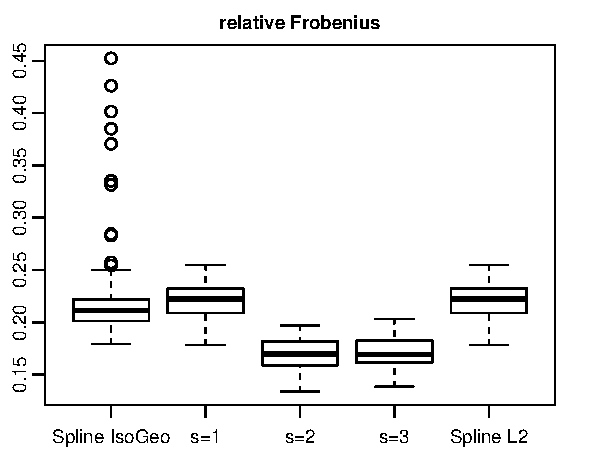
\includegraphics[width=0.3\textwidth]{./graphics/sce=2_SNR=high_Kobs=30_MSE}
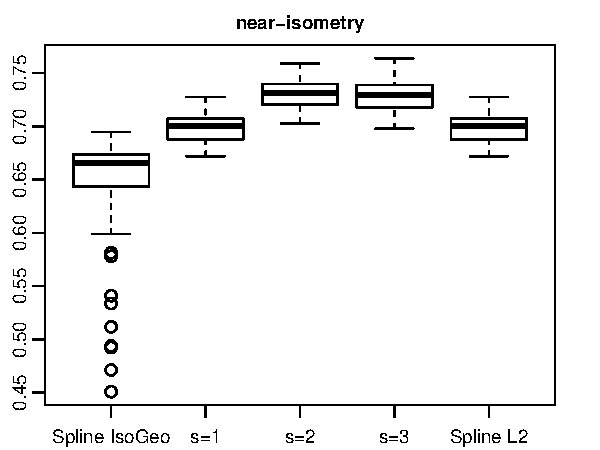
\includegraphics[width=0.3\textwidth]{./graphics/sce=2_SNR=high_Kobs=30_isometry}
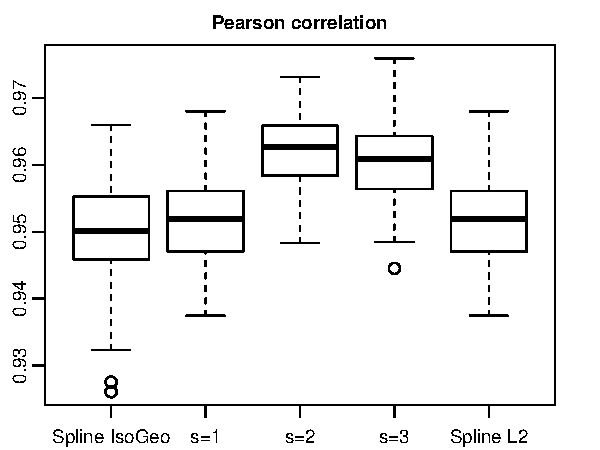
\includegraphics[width=0.3\textwidth]{./graphics/sce=2_SNR=high_Kobs=30_Pearson}
\caption{Manifold of $N(\beta,1)$ probability density functions. The boxplots indicate the distributions of each of the three metrics over 100 Monte Carlo samples. Across all three metrics, our method with $s=2$ performs the best, followed by our method with $s=3$.}
\label{fig:normal}
\end{figure}

\begin{figure}
\centering
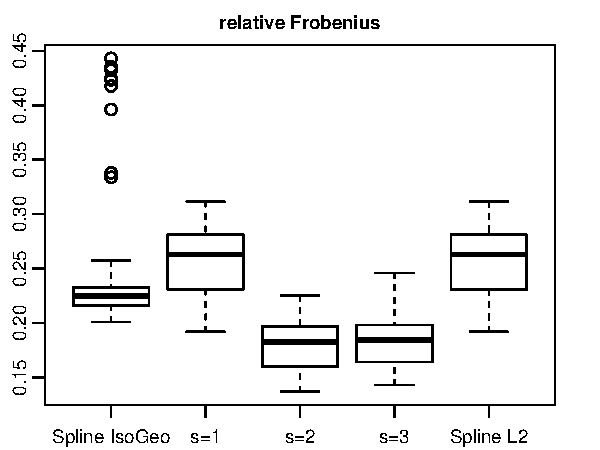
\includegraphics[width=0.3\textwidth]{./graphics/sce=5_SNR=high_Kobs=30_MSE}
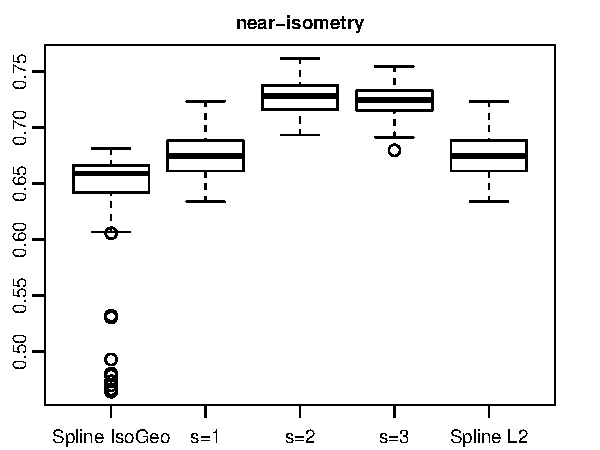
\includegraphics[width=0.3\textwidth]{./graphics/sce=5_SNR=high_Kobs=30_isometry}
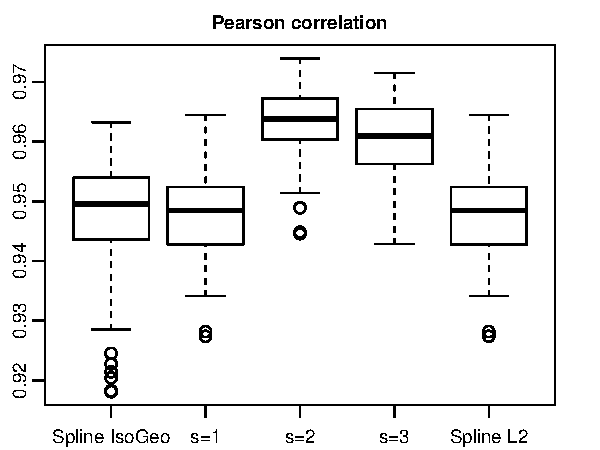
\includegraphics[width=0.3\textwidth]{./graphics/sce=5_SNR=high_Kobs=30_Pearson}
\caption{Manifold of warped functions. The boxplots indicate the distributions of each of the three metrics over 100 Monte Carlo samples. The best performing estimators are given by our method with $s=2$ and then $s=3$.}
\label{fig:warping}
\end{figure}

\begin{figure}
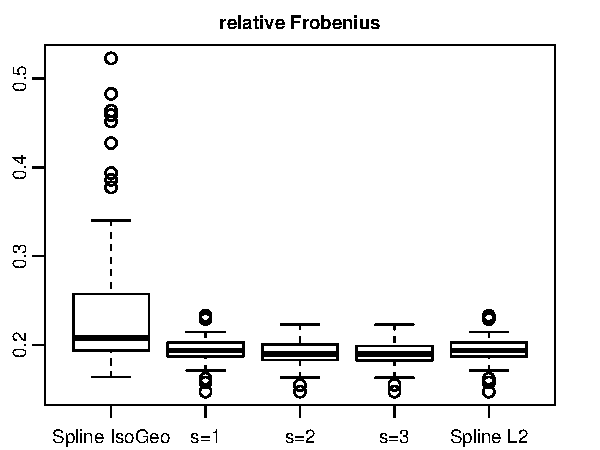
\includegraphics[width=0.3\textwidth]{./graphics/sce=4_SNR=high_Kobs=30_MSE}
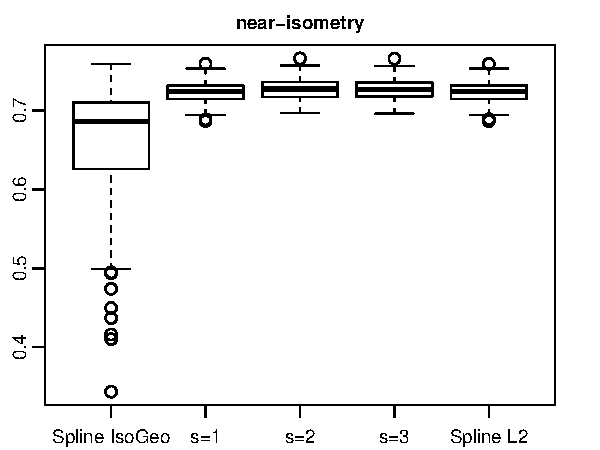
\includegraphics[width=0.3\textwidth]{./graphics/sce=4_SNR=high_Kobs=30_isometry}
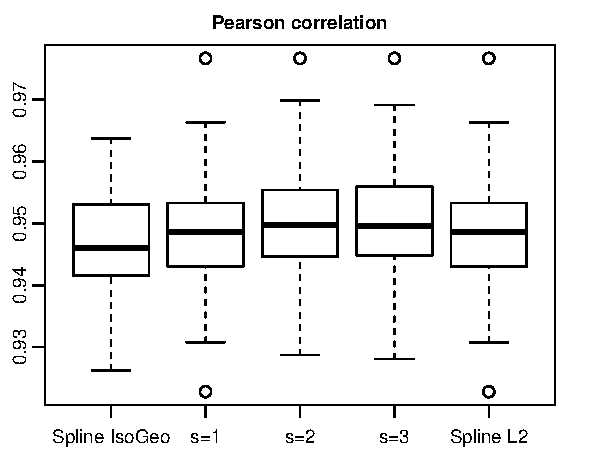
\includegraphics[width=0.3\textwidth]{./graphics/sce=4_SNR=high_Kobs=30_Pearson}
\caption{Manifold of square root Beta densities. The boxplots indicate the distributions of each of the three metrics over 100 Monte Carlo samples. Besides Spline IsoGeo, all methods perform comparably well.}
\label{fig:betas}
\end{figure}

\section{Conclusion}


\section{DISTANCE-BASED FUNCTIONAL CLASSIFICATION}\label{distance-based-functional-classification-marie}

There are many downstream analysis tasks in functional data analysis that are based on pairwise distances, including distance-based nonparametric regression and distanced-based functional clustering.
In this section, we explore whether our geodesic distance estimator has
benefits for the downstream analysis task of functional classification. 

We work with the non-parametric classifier proposed in \cite{Ferraty2006} which is a functional version of the Nadaraya-Watson kernel estimator. Given a sample of curves $X_1,\ldots,X_n$ where each function $X_i$ is associated to a class label $Y_i$, the estimator of the probability that a new observation $X^\star$ is in class $Y^\star=y$ is defined as
\begin{equation}\label{func_NW}
\hat P(Y^\star = y | X^\star)= \frac{ \sum_{i=1}^n k[h^{-1} d(X^\star,X_i)] {\bf{1}}(Y_i = y) }{ \sum_{i=1}^n k[h^{-1} d(X^\star,X_i)] },
\end{equation}
where $d$ is a distance, $k$ a kernel, $h$ a bandwidth and $\bf{1}$ the indicator function. The curve $X^\star$ is then classified in the class $Y^\star =y$ for which the conditional probability (\ref{func_NW}) is largest. We compare the classification performance obtained with the distance $d$ given by our proposed geodesic distance with $s=1,2$ and $3$, as well as that given by Spline IsoGeo and Spline L2 described in the simulation study section. We set $k$ to be a quadratic kernel and the bandwidth $h$ is chosen by cross-validation. 

The classification task is performed on the well-known Berkeley growth curves dataset in functional data analysis, available in the \emph{fda} package \cite{Ram-Hoo-Gra} for R \cite{Rproject}. We chose this dataset because we expect the data to contain nonlinear features as suggested in \cite{ChenMuller2012}. The data consist of the height of $n=93$ individuals, 39 boys and 54 girls, measured on a common grid $t_1,\ldots,t_K$ of $K=31$ points taken between the ages of 1 and 18 years. The raw data $Y_1,\ldots,Y_n$ are transformed to continuous functions by smoothing with B-spline bases with a roughness penalty on the fourth derivative :
$$\tilde X_i(t) = \sum_{l=1}^{b} c_{il}B_l(t), $$
where
 \begin{eqnarray*}
 (c_{i1},\ldots,c_{ib})&=&\arg \min_{c\in \R^b}\Bigg\{\sum_{j=1}^K\left(\sum_{l=1}^{b} c_{il}B_l(t_j)-Y_{ij}\right)^2\\
 &&\quad +\lambda \left\|\sum_{l=1}^{b} c_{il}\partial^4_tB_l\right\|^2_{L^2}\Bigg\}.
 \end{eqnarray*} 
We use $b=35$ B-splines bases of order 6 and the parameter $\lambda$ is chosen by generalized cross-validation. We then differentiate the resulting fonctions to obtain velocity curves; the data are illustrated for boys and girls on Figure \ref{fig:data_illu}.





To assess the classification performance of the the proposed geodesic distance, we randomly split $200$ times the dataset into a training set of $50$ curves and a test set of $43$ curves. For each split, we calculate the misclassification error, and we average these errors over the splits. The results are presented in Figure \ref{fig:class_err_velo}, we can see that our method with $s=3$ performs a little bit better than the others and that our method with $s=2$ is equivalent to Spline IsoGeo and Spline L2.

\begin{figure}[t]
\centering
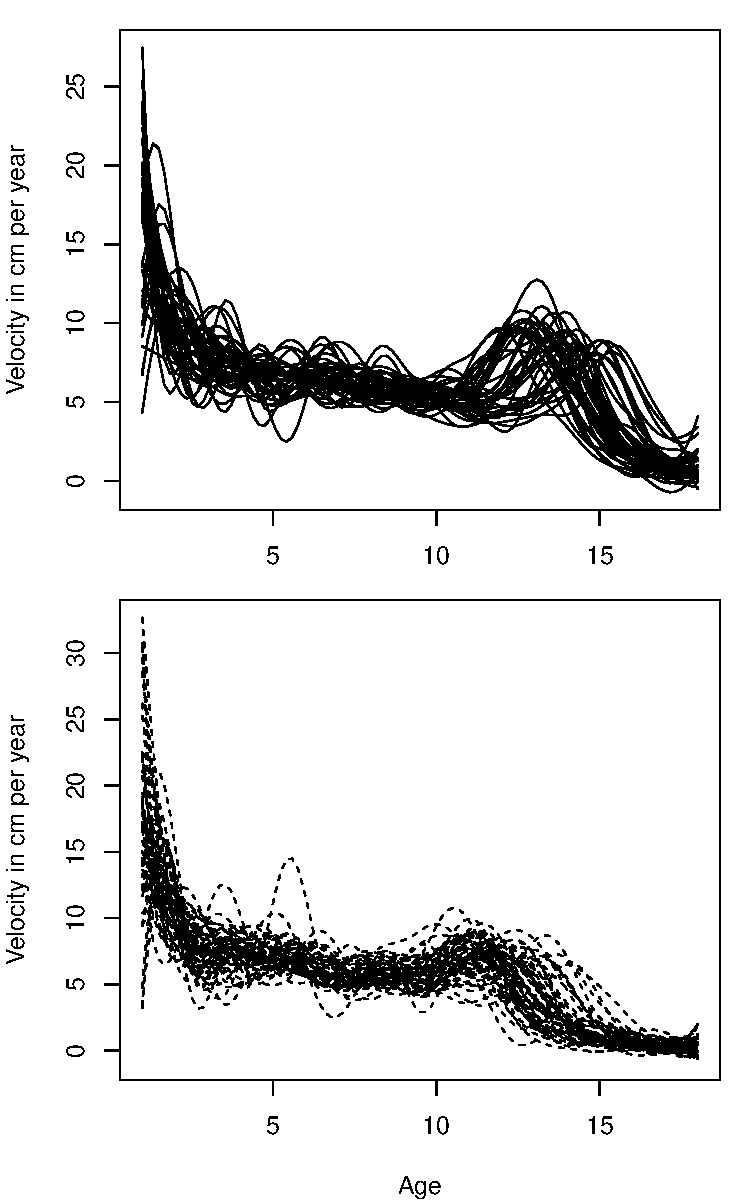
\includegraphics[height=0.5\textheight]{./Velocity_curves_data_illustration.pdf}
\caption{Velocity curves of 39 boys (top) and 54 girls (bottom).}
\label{fig:data_illu}
\end{figure}

\begin{figure}[h!]
\centering
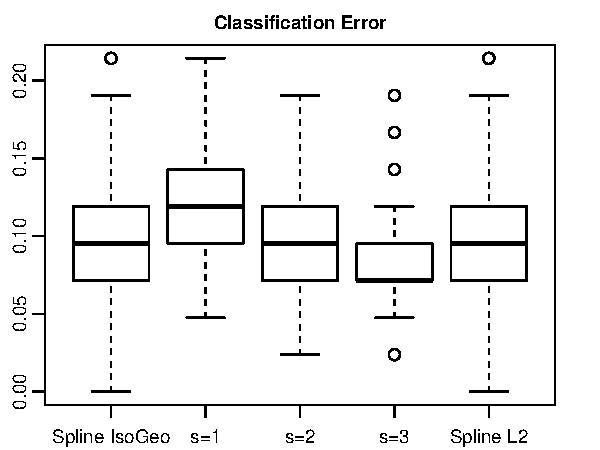
\includegraphics[height=0.3\textheight]{./Erreur_classification_velocity.pdf}
\caption{Classification errors for the velocity curves, our method with $s=3$ performs better while our method with $s=2$ is equivalent to Spline IsoGeo and Spline L2.}
\label{fig:class_err_velo}
\end{figure}


% It must be noted that while
% curve alignment, also known as curve registration, is necessarily
% performed as a preprocessing technique prior to clustering and
% classification, our geodesic distance estimator allows one to forsake
% this step.




 


% For simplicity, assume the task is binary classification. Associated to
% each functional object \(x\) is a binary \(y\) indicating class
% membership. Consider the classifier proposed in \cite{Ferraty2006} which
% is a functional version of the Nadaraya-Watson kernel estimator of class
% membership probabilities: \[
% \hat p(y = 0 | x) \frac{ \sum_{i=1}^n K[h^{-1} d(x,x_i)] 1(y_i = 0) }{ \sum_{i=1}^n K[h^{-1} d(x,x_i)] }
% \] We shall compare our method to using \(L^2\) distance, possibly
% weighted, and with curve registration already accomplished. Describe
% alternative methods in detail.
% 
% The bandwidth in the classifier should be tuned individually for each
% method. Also we might need to tune MDS dimension \(s\) since in real
% data, the dimension of the manifold might be much higher than
% encountered in the simulation scenarios where it never goes above 2.

% Datasets used by functional classification papers
% 
% \begin{itemize}
% \item Wheat, rainfall and phoneme in Aurore's paper "Achieving near-perfect classification for functional data"
% \item Berkeley growth curves in \cite{ChenReiss2014}.
% \item Tecator and phoneme in \cite{Galeano2015} Mahalanobis technometrics paper.
% \item yeast cell cycle gene expression (can't find this publicly) in \cite{LengMuller2005} "Classification using functional data analysis for temporal gene expression data"
% \end{itemize}
% 
% Datasets used in functional manifold papers
% 
% \begin{itemize}
% \item Berkeley growth, yeast cell cycle gene expression (can't find this publicly) in \cite{ChenMuller2012}
% \item Tecator in \cite{LinYao2017} contamination paper
% \item Berkeley growth, gait cycle in \cite{Dimeglio2014} robust isomap paper
% \end{itemize}


%\backmatter

\section*{Acknowledgments}
This is acknowledgment text~\cite{Elbaum2002}. Provide text here. This is acknowledgment text. Provide text here. This is acknowledgment text. Provide text here. This is acknowledgment text. Provide text here. This is acknowledgment text. Provide text here. This is acknowledgment text. Provide text here. This is acknowledgment text. Provide text here. This is acknowledgment text. Provide text here. This is acknowledgment text. Provide text here. 

\subsection*{Author contributions}

This is an author contribution text. This is an author contribution text. This is an author contribution text. This is an author contribution text. This is an author contribution text. 

\subsection*{Financial disclosure}

None reported.

\subsection*{Conflict of interest}

The authors declare no potential conflict of interests.


\section*{Supporting information}

The following supporting information is available as part of the online article:

\noindent
\textbf{Figure S1.}
{500{\uns}hPa geopotential anomalies for GC2C calculated against the ERA Interim reanalysis. The period is 1989--2008.}

\noindent
\textbf{Figure S2.}
{The SST anomalies for GC2C calculated against the observations (OIsst).}


\appendix

\section{Section title of first appendix\label{app1}}



%\nocite{*}% Show all bib entries - both cited and uncited; comment this line to view only cited bib entries;
\bibliography{references.bib}%


\section*{Author Biography}

\begin{biography}{
\includegraphics[width=60pt,height=70pt,draft]{empty}}{\textbf{Author Name.} This is sample author biography text this is sample author biography text this is sample author biography text this is sample author biography text this is sample author biography text this is sample author biography text this is sample author biography text this is sample author biography text this is sample author biography text this is sample author biography text this is sample author biography text this is sample author biography text this is sample author biography text this is sample author biography text this is sample author biography text this is sample author biography text this is sample author biography text this is sample author biography text this is sample author biography text this is sample author biography text this is sample author biography text.}
\end{biography}

\end{document}
